\section{Modeller}

Her følger uformell dokumentasjon over dataevolusjonsmoculen DBUpgradinator og hvordan den skal oppføre seg i en datadreven webapplikasjon hvis dataelementer persisteres i en distribuert database. Dokumentasjonen er basert på 4+1-metamodellen Phillippe Kruchten presenterer i en artikkel fra 1995.

\subsection{4+1 - stilen}

Dokumentasjon av programvarearkitektur er en kommunikasjonskunst. Symbolene som tegnes på et lerret eller på en bildefil bærer ingen betydning eller mening i seg selv, hva de representerer er noe dokumentets forfattere og dets påtenkte publikum må være samstemte om. Videre er tydelige kommuniserende begrenset når det kommer til hvor mange konsepter de kan representere på ett og samme tidspunkt. En firkant, eller en boks, kan til eksempel ikke representere både en statisk fil med programkode i og samtidig en kjørende prosess.

Enkelte arkitekturdokumenter fokuserer for mye på ett enkelt aspekt ved datasystemet, eller tar ikke hensyn til ønsker og bekymringer til samtlige interessenter, de distinkte gruppene som leser dokumentet. Derfor foreslår \cite{kruchten1995} å organisere dokumentasjonen til en programvarearkitektur inn i en mengde av fire perspektiv (eng. viers) som hver for seg besvarer ett spesifikk interesseområde for applikasjonen.

Disse fire perspektivene kaller \cite{kruchten1995} for:
\begin{description}
  \item [Det logiske perspektivet] I kontekst av objekt-orientert programmering er dette en oversikt over objekter (teknisk sett prosesser/tråder) som eksisterer i primærminnet til datamaskinene i systemet
  \item [Prosessperspektivet] Gir leseren en oversikt over detaljer angående samtidige operasjoner og synkronisering i systemets design
  \item [Det fysiske perspektivet] Beskriver 1) koplingene mellom programvareelementer og maskinvareelementer i systemet og 2) systemets distribuerte naturBeskriver 1) koplingene mellom programvareelementer og maskinvareelementer i systemet og 2) systemets distribuerte natur
  \item [Utviklingsperspektivet] Beskriver programvarens statiske organisering av dets kildekode i utviklermiljøet
\end{description}

Den primære oppgaven til det logiske perspektivet av arkitekturdokumentasjonen er å representere effektene de funksjonelle krav som stilles til datasystemet har på det. De funksjonelle krav har opprinnelse i domenet til problemet datasystemet angriper. Systemets viktigste abstrakte konstruksjoner, kalt objekter i programmets og klasser i kildekoden, kan knyttes til separate begreper inneholdt i domenet til problemet interessentene (de som leser arkitekturdokumentet) vil løse \citep{kruchten1995}. Objekter utnytter egenskaper som arv/spesialisering, innkapsling og funksjonsmaskering gjennom grensesnitt for å realisere påkrevd funksjonalitet.

Logiske perspektiver inneholder gjerne klassediagrammer og sekvensdiagrammer skrevet med UML - syntaksen. Et klassediagram viser en oversikt over klassene og relasjoner mellom dem i et objekt-orientert program. Hvis applikasjonen er sterkt datadrevet, slik tilfelle gjerne er i kommersielle webapplikasjoner som netthandel-informasjonssystemer, er det hensiktsmessig å presentere et ER -  eller et EER - diagram i det logiske perspektivet også.

Prosessperspektivet beskriver hvordan oppfører seg når det kjører og hvordan det kjører. Prosessperspektivet reflekterer de ikke-funksjonelle krav, herunder kvalitetskrav, krav til systemoppførsel og begrensende krav, som stilles til datasystemet. Sentrale problemer som tas stilling til inkluderer samtidighet, feiltoleranse, distribusjon av arbeidslast, integritet, parallelt kjørende tråder og hvordan entiteter, klasser eller objekter fra det logiske perspektivet gjenspeiles i prosessperspektivet \citep{kruchten1995}.

Her svarer et objekt fra det logiske perspektivet til en tråd underordnet en kjørende prosess i et operativsystem. Et høytilgjengelig system vil typisk modelleres slik at enhver slik prosess i systemet har en identisk tvilling som kan steppe inn og ta over sin partners arbeidslast skulle den svikte, også kjent som en reserveprosess, på engelsk kalt for ‘’spare’’.

Oppgaven til programvarearkitekturdokumentasjonens fysiske perspektiv er å definere sammenhengen mellom kildekode og maskinvaren (m.a.o. datamaskiner) som koden kjører på. Perspektivet er særskilt relevant for systemer der strenge, spesifikke krav stilles dets ytelse (gjennomstrømming i fore eksempel antall transaksjoner per sekund), tilgjengelighet (evnen til å handtere delvis eller fullstendig svikt) og pålitelighet (feiltoleranse).

Arkitekturen til et distribuert system består av et nettverk av uavhengige datamaskiner som prosesserer data, kalt \emph{noder}. Derfor er det vesentlig å dokumentere hvilken rolle de abstrakte programvareelementer fra prosessperspektivet og utviklingsperspektivet spiller i forhold til de forskjellige fysiske noder \citep{kruchten1995}.

Systemet har vanligvis forskjellige konfigurasjoner, en mengde parametere som bestemmer programvarens oppførsel under kjøretid. Én konfigurasjon kan gjelde for systemets testfase, en annen for når dets produksjonsmiljø, og et atter annet for vedlikeholds- eller utviklingsmiljø \citep{kruchten1995}. De forskjellige konfigurasjoner illustreres ofte i hvert sitt distribusjonsdiagram, som også kan skisseres med UML-syntaks.

Utviklingsperspektivet tiltaler primært applikasjonens utviklere og vedlikeholdere, de som skal endre dets kildekode. Programmet inndeles i mindre enheter, kalt ‘’bibliotek’’ eller ‘’moduler’’, hvilket kan refereres til og benyttes av utviklere på tvers av store eller små prosjektgrupper. Disse modulene er organisert hierarkisk i forskjellige \emph{lag}, det vil si at hver modul eksponerer et veldefinert programmeringsgrensesnitt som andre moduler organisert direkte over den kan kalle på uten å være involvert i bibliotekets kildekode.

Diagrammer innen utviklingsperspektivet viser derfor typisk import/eksport - forhold imellom forskjellige programvaremoduler, som i tur også kan samles sammen inn i pakker, som best kan beskrives som ‘’meta-moduler’’. Selv om utviklingsperspektivet ikke er komplett før samtlige programvareelementer i systemet er definert og navngitt kan det deklarere de regler som bestemmer kildekodeorganiseringens natur, deriblant eksponering av funksjoner via import/eksport av bibliotek, gruppering av moduler inn i pakker, og avgrensning av moduler. Utviklingsperspektivet er nyttig primært for ansvarsfordeling og å gjøre konkrete implementasjonsvalg som valg av språk, utviklingsverktøy og tredjepartsmoduler lettere.

Disse fire separate perspektivene kan også kombineres sammen i et femte perspektiv, kalt bruksscenarier, som oppsummerer systemets mengde av funksjonelle krav \citep{kruchten1995}. Meningen bak dekomponeringen av programvarearkitekturdokumentasjonen er å belyse vesentlige interesseområder av systemet. Det er vesentlig å notere at perspektivmodellen i all hovedsak er en metamodell - en beskrivelse av sammenhengen mellom konkrete modeller for programmet brukt i arkitekturens dokumentasjon.

Videre må det nevnes at samtlige perspektiver i metamodellen er valgfrie, enhver arkitekt står fri til å gjøre justeringer på sitt dokument i henhold til de krav som stilles systemarkitekturen som modelleres. DBUpgradinator modelleres med de tre første perspektivene i 4+1-metamodellen. Ettersom prosjekter er et enmannsarbeid er et sett av diagrammer som utgjør et eget utviklingsperspektiv ikke strengt nødvendig. Ett perspektiv som i kontekst av distribuerte applikasjoner er uunnværlig er det fysiske perspektivet.

\subsection{Det logiske perspektiv}
% Figur 5
\begin{figure}[hbtp]
    \centering
    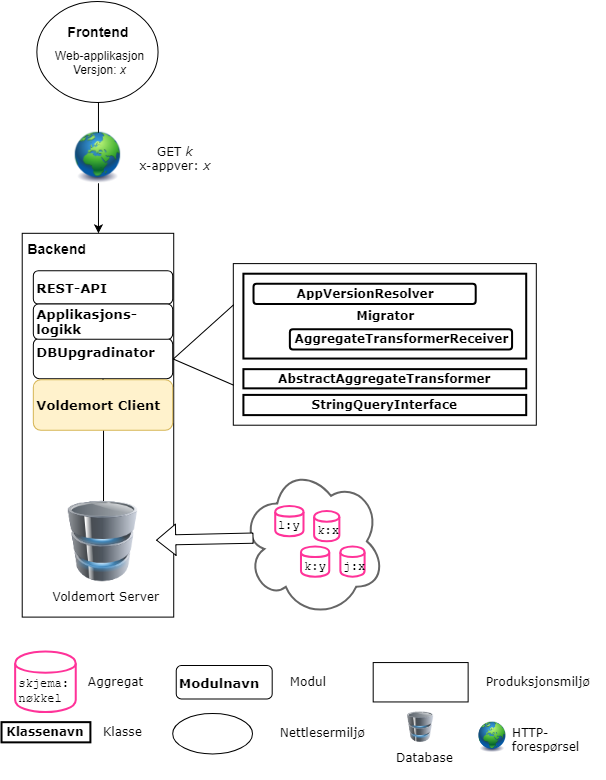
\includegraphics[scale=0.6]{fig/dbupgradinator-logisk-1.png}
    \caption{Logisk oversikt over moduler i det typiske produksjonsmiljøet DBUpgradinator opererer i. Klassene som DBUpgradinator består av nevnes med navn.}
    \label{fig5}
\end{figure}

Figur \ref{fig5} viser en oversikt over de ulike bestanddelene i DBUpgradinator. Figuren viser også DBUpgradinator sin logiske relasjon til REST-webapplikasjonen brukt til å teste dette migrasjonsverktøyet i. Det logiske perspektivet (eng. ''view'') beskriver også de ulike atomiske moduler webapplikasjonen består av.

Webapplikasjonen er inndelt i to nivå: Ett nivå for visningslogikken (''Frontend'') og ett for tjenerlogikken (''Backend''). Visningslogikken kjøres i et nettlesermiljø, det vil si at visningslogikken er en nettside som åpnes av en nettleser, som Microsoft Edge eller Mozilla Firefox. Nettleseren viser elementer som dikteres av kildekoden til siden nettleseren åpnet. ''Frontend'' - miljøet i diagrammet markeres med en sirkel fordi det er et klientprogram, separat fra tjenerne, som kjører i en nettleser. Intensjonen med webapplikasjonen er at det er nettlesere som skal kjøre klientprogrammet. Frontendklienten oppretter og sender HTTP-forespørsler til det funksjonelle grensesnittet til applikasjonstjeneren.

Tjenerlogikken instansieres og kjøres innenfor et kjøretidssystem (eng. ''run-time system''), en spesialisert programvare som implementerer deler av kjøringsmodellen til et språk. En kjøringsmodell skisserer hvordan kode kjøres i et operativsystemet, for eksempel kan den være event-basert og tillate asynkron kjøring av kode, slik tilfelle er med kjøretidssystemet NodeJS. Fra et operativsystem sitt perspektiv anskues kjøretidssystemet som en selvstendig prosess. Det kommuniserer med operativsystemets grensesnitt på vegne av programmet det instansierer og kjører som en tråd underordnet seg selv. Kjøretidsmiljøet til Java heter for Java Runtime Environment (JRE).

Figur \ref{fig5} viser hvordan den logiske strukturen til webapplikasjoner, som DBUpgradinator er skrevet for, skal se ut. Applikasjonstjeneren består av følgende elementer:

\begin{description}
  \item [REST-API] er applikasjonsgrensesnittet visningslogikken kommuniserer med via HTTP. De fire typiske kommandoene grensesnittet betjener er HTTP-verbene \texttt{GET}, \texttt{PUT}, \texttt{POST} og \texttt{DELETE}.
  \item [Applikasjonslogikken] til webapplikasjonen er kode som behandler HTTP-forespørsler og oppretter HTTP-responser. Den videresender både skjemanøkkel og aggregatnøkkel ned til DBUpgradinator, som handterer og besvarer spørringen.
  \item [DBUpgradinator] - Programmet som migrerer hvert aggregat, asynkront fra brukerforespørsler.
  \item [VoldemortClient] er klientprogrammet til Project Voldemort. Det utfører databasekall til \(N\) databasenoder. VoldemortClient er også ansvarlig for å kontrollere aggregatenes vektorklokke\-versjoner når den mottar spørringsresultater fra av hver av disse nodene før den returner et endelig spørreresultat. Ved skriveoperasjoner venter klienten på \(W\) bekreftelser før den besvarer applikasjonen. Ved leseoperasjoner  venter klienten på \(R\) bekreftelser. 
  \item [Voldemort Server] - Én eller flere databaseprosesser som lagrer og henter data.
\end{description}

DBUpgradinator består av følgende elementer, som vist i boksen til høyre i figur \ref{fig5}:

\begin{description}
  \item [Migrator] er det objektet i pakken som utfører alle spørringer mot databasen, både for å betjene brukerforespørsler, og for å persistere migrerte aggregater, opprettet av \textbf{Abstract}\-\textbf{Aggregate}\-\textbf{Transformer}-objektet på strengformat. Derfor er DBUpgradinator modellert som et eget lag i webapplikasjonens logiske stakk, plassert under appliaksjonslogikken og over databasegrensesnittet ''VoldemortClient'', i figur \ref{fig5}.
  \item [AggregateTransformerReceiver] er en modul som mottar et \textbf{AbstractAggregateTransformer} - objekt via en I/O-operasjon, og holder rede på det i programminnet.
  \item [AppVersionResolver] Oppgaven til denne modulen er å kople dataobjektets nøkkel i en innkommende HTTP-spørring (k) med applikasjonsversjonens nøkkel (x) på formen \texttt{k + '':'' + x}
  \item [AbstractAggregateTransformer] er et objekt som transformer aggregater som enten er mottatt fra en HTTP-forespørsel (PUT eller POST) eller mottatt fra databasen som et resultat av en GET-forespørsel. Selve transformasjonsfunksjonen er implemtert av applikasjonens utviklere eller vedlikeholdere.
  \item [StringQueryInterface] Modul som sender GET og PUT - spørringer for Migrator-objektet til ''VoldemortClient''.
\end{description}

% Figur 6
\begin{figure}[hbtp]
  \centering
  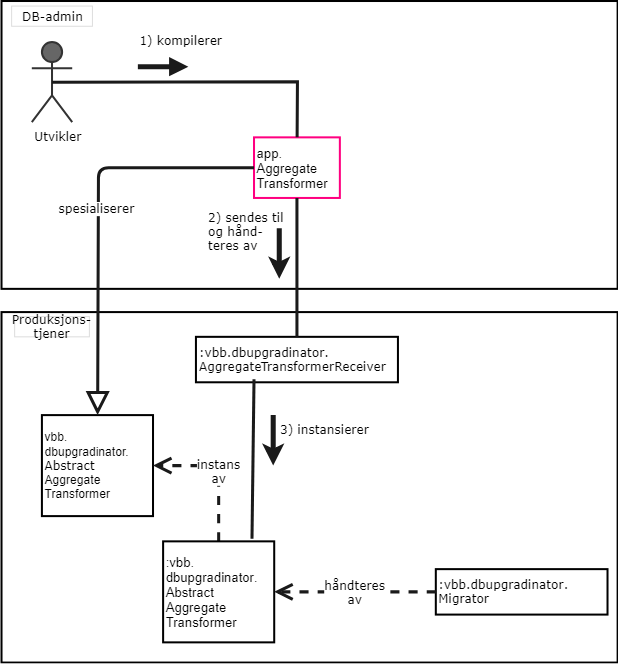
\includegraphics[scale=0.6]{fig/dbupgradinator-logisk-2.png}
  \caption{Kommunikasjonsdiagram som illustrerer forholdet mellom en utvikler og en applikasjonstjener der DBUpgradinator benyttes for å migrere data levende.}
  \label{fig6}
\end{figure}

Figur \ref{fig6} forteller oss hvem det er som har ansvar for å skrive aggregat\-transformasjonsklassen, nemlig aktøren kalt ''Utvikler'', som har ansvar for migrasjonen av data i en databaseinstans. Akkurat som i KVolve, er det den enkelte applikasjonsutvikler som må definere aggregat\-transformasjons\-funksjonen fordi de både har kunnskap om domenet applikasjonen opererer i, og hvordan datamodellen til applikasjonen utvikler seg i takt med kildekodens endringer.

Etter å ha implementert transformasjonsklassen (markert med rosa omriss i kommunikasjonsdiagrammet) som spesialiserer \textbf{AbstractAggregateTransformer}, kompilerer utvikleren filen til en \texttt{.class} - fil og sender den til hver applikasjonstjener som kjører i systemet. AggregateTransformerReceiver-modulen leser inn alle oktettene i filen tjeneren mottar, inn en byte-matrise og skaper et objekt i minnet. Dette objektet opprettes som en instans av \textbf{AbstractAggregateTransformer}. Dette objektet blir dernest plassert i \textbf{Migrator}-instansens liste av transformatorer. I \ref{fig6} er objektinstanser merket med kolon i navnet.

\subsection{Prosessperspektivet}

% Figur 7
\begin{figure}[hbtp]
  \centering
  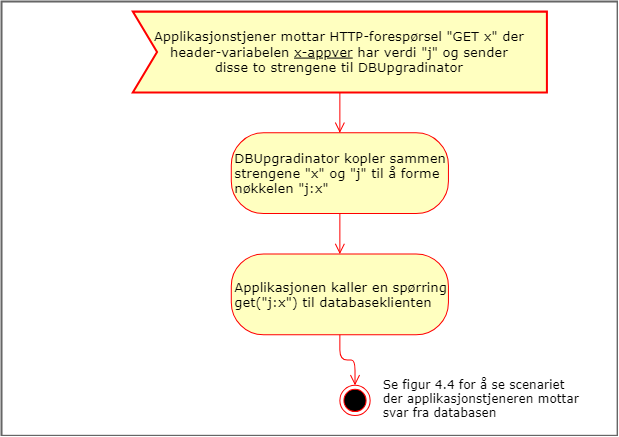
\includegraphics[scale=0.8]{fig/dbupgradinator-prosess-1.png}
  \caption{Aktivitetsdiagram som illustrerer hvordan DBUpgradinator interfererer i applikasjonslogikken ved en \texttt{GET} - forespørsel før databaseklienten mottar spørringen.}
  \label{fig7}
\end{figure}

Aktivitetsdiagrammet i figur \ref{fig7} beskriver systemets oppførsel når en GET-forespørsel fra en applikasjonstjener hvis skjemaversjon er j, mens produksjonsmiljøet er under oppgradering av dataskjemaet fra versjon \emph{j} til \emph{k}, der \emph{k} etterfølger \emph{j}. Applikasjonsjeneren kaller på AppVersionResolver\-modulen i DBUpgradinator for å sette sammen aggregatets nøkkel med dataskjemanøkkelen. Dernest kaller tjeneren på \texttt{get} - metoden til en StoreClient - instans. Tråden som utførte dette databasekallet vil da bli blokkert.

% Figur 8
\begin{figure}[hbtp]
  \centering
  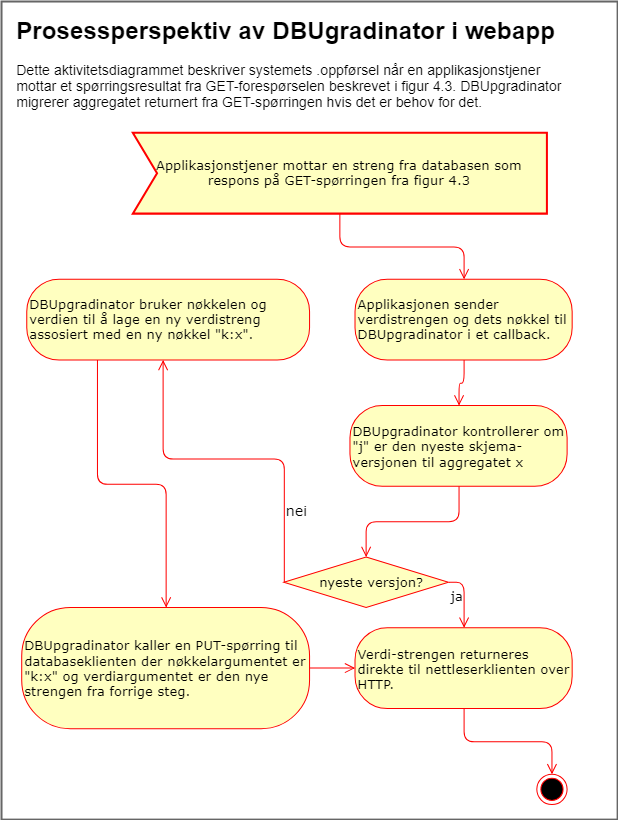
\includegraphics[scale=0.6]{fig/dbupgradinator-prosess-2.png}
  \caption{Aktivitetsdiagram som illustrerer hvordan DBUpgradinator interfererer i applikasjonslogikken ved en \texttt{GET} - forespørsel etter at spørringen er ferdig.}
  \label{fig8}
\end{figure}

Aktivitetsdiagrammet i figur \ref{fig8} beskriver systemets oppførsel når applikasjons\-tjener\-tråden mottar resultatet fra GET-forespørselen beskrevet i figur \ref{fig7}. DBUpgradinator migrerer aggregatet returnert fra GET-spørringen hvis det er behov for det. Når applikasjonen mottar et aggregat fra VoldemortClient, sender den både aggregatet og nøkkelen til DBUpgradinator.

Pakken kontrollerer om aggregatet er av den nyeste skjemaversjonen, det vil si at det ikke finnes noen transformatorobjekt hvis ''nå''-versjon tilsvarer aggregatets skjemaversjon. Hvis dette er tilfelle, overlater DBUpgradinator eksekveringskontroll tilbake til applikasjonstjeneren direkte, som putter aggregatet inn i body-feltet til en HTTP-respons, som til slutt sendes tilbake til applikasjonsklienten.

I det motsatte tilfelle sender programmet aggregatet inn i transformasjonsfunksjonen, som lager en ny streng utifra strengargumentet den fikk tilsendt. Ved hjelp av prosessen \emph{AppVersionResolver} lager programmet en ny nøkkel der skjemaversjon\-suffikset tilsvarer den strengen transformatorobjektet indikerer er navnet på det neste skjemaet. Dernest sendes en ny databasespørring der det migrerte aggregatet opprettes/oppdateres (put-kall) på den nye nøkkelen, fra en separat tråd enn den som betjener den brukerinitierte forespørselen. Med en gang databasespørringen til det migrerte aggregatet tilsendes StoreClient, returneres spørreresultatet til applikasjonstjeneren.

% Figur 9
\begin{figure}[hbtp]
  \centering
  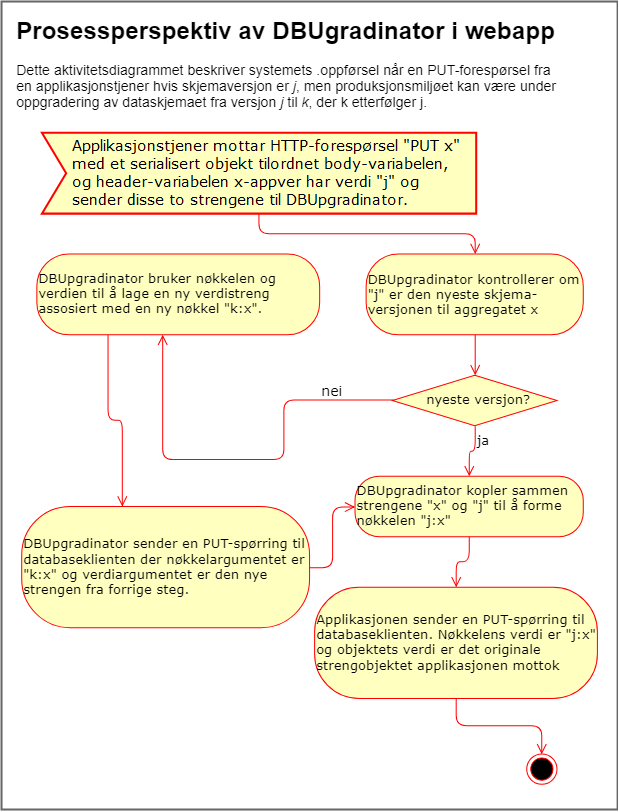
\includegraphics[scale=0.6]{fig/dbupgradinator-prosess-3.png}
  \caption{Aktivitetsdiagram som illustrerer hvordan DBUpgradinator påvirker applikasjonens oppførsel ved en innkommende \texttt{PUT} - forespørsel.}
  \label{fig9}
\end{figure}

Aktivitetsdiagrammet i figur \ref{fig9} beskriver webapplikasjonens oppførsel når en PUT-forespørsel fra en applikasjonstjener hvis skjemaversjon er \emph{j}, mens produksjonsmiljøet er under oppgradering av dataskjemaet fra versjon \emph{j} til \emph{k}, der \emph{k} etterfølger \emph{j}.

Forretningsordenen for en skriveforespørsel er omvendt av den vi så for leseforespørsler i figurene \ref{fig7} og \ref{fig8}. Her blir DBUpgradinator kontaktet før databasespørringen sendes. Årsaken er at aggregatet ved PUT eller POST er gitt av klienten, sammen med både dets påtenkte skjema og dets statiske nøkkel. Igjen vil DBUpgradinator kontrollere skjemaversjonen, og asynkront migrere aggregatet ved å opprette en ny streng basert på det, hvis skjemanøkkelen som kommer fra forespørselen ikke er den nyeste. Etter å ha utført migrasjonen av det oppdaterte aggregatet og sendt resultatet til databaseklienten i form av et put-funksjonskall, hopper programmet tilbake inn i applikasjonslogikken, og sender et nytt put-kall til samme databaseklient.

Dette databasekallet gjøres for å oppdatere det objektet som i prinsippet er det samme aggregatet, men for det gamle skjemaet. Årsaken til at DBUpgradinator oppdaterer aggregatet for det nye skjemaet, samtidig som for det gamle, er at ved rullerende oppgradering av en klynge applikasjonstjenere har man en miks av tjenere som opererer med den gamle versjonen av tjenerprogrammet og tjenere som kjører den nye. Mengden av nye tjenerversjoner øker gradvis på bekostning av mengden av de gamle, naturlig nok, ved en rullerende applikasjonsoppdatering.

Når applikasjonen mottar en bekreftelse fra et put-kall opprettes en HTTP-respons som informerer om hvorvidt skriveoperasjonen lyktes eller ikke. Responsen sendes tilbake til applikasjonsklienten over TCP/IP - forbindelsen.

\subsection{Det fysiske perspektiv}

% Figur 10
\begin{figure}[hbtp]
  \centering
  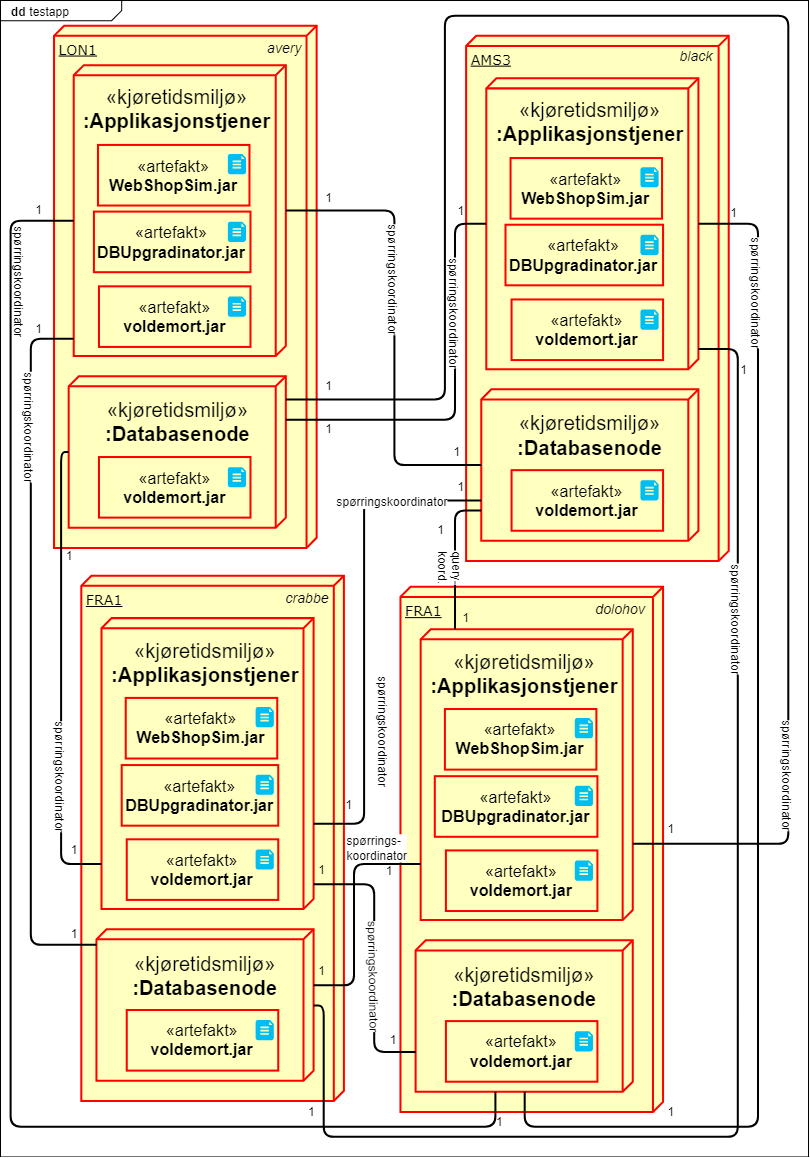
\includegraphics[scale=0.4]{fig/dbupgradinator-physical.png}
  \caption{Deployment-diagram av webapplikasjonen DBUpgradinator testes i.}
  \label{fig10}
\end{figure}

De fire boksene i figur \ref{fig10} refererer til fire forskjellige datasentre. Hver enkelt av de fire applikasjonsnodene gjestes av skyinfrastrukturleverandøren DigitalOcean, og alle er spredd utover fire forskjellige datasentre i London, Amsterdam (to av datasentra er lokaliserte her), og Frankfurt am Main.

I hvert datasenter betjenes én virtuell maskin, eller \underline{droplet}, som DigitalOcean kaller dem. Selve maskinvaren blir beskrevet i detalj i delkapittel 5.3. Hver av de virtuelle maskinene kjører to separate programmer (''kjøretidsmiljø'') som lytter på én nettverksport hver. Disse programmene er:

\begin{enumerate}
  \item Webapplikasjonen, som i \ref{fig10} benytter artefaktene WebShopSimulator.jar og DBUpgradinator.jar til å kjøre selve appliaksjonstjeneren; samtidig benytter prosessen voldemort.jar - filen for å instansiere en klient som replikerer hvert aggregat til tre databasenoder
  \item Databasenoden, som lagrer og henter data på kommando fra Voldemort-klientprogrammene
\end{enumerate}

Figur \ref{fig10} viser også at hver kjørende instans av Voldemort-klienten fra applikasjonstjenerprogrammet har én replikeringsassosiasjon med hver av de tre databasenodene stasjonert på de andre virtuelle maskinene. Det er ikke nødvendigvis slik hash-strategien er konfigurert i databaseinstansen, figuren er ment å illustrere at klientprogrammet til Voldemort er del av applikasjonsprosessen, og det er den som utførerer spørringer mot de enkelte databasenoder for å persistere og lese repliaker.

